\chapter{HASIL DAN PEMBAHASAN}
\label{chap:hasil dan pembahasan}

% Ubah bagian-bagian berikut dengan isi dari pengujian dan analisis

Pada penelitian ini dilakukan 3 aspek pengerjaan dalam menjawab tujuannya, diantaranya adalah data eksperimen yang telah didapatkan dari PTDI. Kemudian validasi matematis menggunakan landasan teori yang telah disesuaikan dengan kondisi pengerjaan penelitian ini, yaitu \textit{ground resonance} helikopter. Kemudian yang terakhir adalah simulasi untuk mendukung hasil data pengukuran dan perhitungan. 

\section{Hasil Data Pengukuran dan Perhitungan}
\label{sec:hasilpengukuran}

\subsection{Hasil pengukuran getaran pada FTIS}

Hasil pengukuran data \textit{ground test} dibagi menjadi 2 bagian, seperti yang telah dijelaskan pada bagian metodologi penelitian, bahwa data yang didapatkan merupakan data pengukuran getaran pada FTIS untuk mencari \textit{damping ratio} dan pengukuran data getaran pada akseleromter untuk mendapatkan respon frekuensi dominan oleh helikopter akibat \textit{input} yang diberikan. Berikut ini merupakan grafik yang didapatkan dari masing-masing kondisi yang mengacu pada tabel \ref{tb:variasilanding}.

\begin{figure}[H]
	\centering
	\fbox{\includegraphics[width=0.7\linewidth]{gambar/FTIS_image/All-plot/All_config_1.jpg}}
	\caption{Grafik data hasil pengukuran kondisi 1.}
	\label{fig:condition_1}
\end{figure}

Selanjutnya merupakan grafik dengan keterangan serupa, dimana pada grafik tersebut memiliki keterangan sebagaimana pada tabel berikut:

\begin{table}[]
	\caption{Keterangan pengukuran pada grafik}
	\begin{tabular}{|c|c|c|}
		\hline
		\textit{Lateral cyclic displacement (\%)} & \textit{Longitudinal cyclic displacement} & Pedal displacement (\%)           \\ \hline
		\textit{Roll (deg)}                       & \textit{Pitch (deg)}                      & \textit{Heading (deg)}            \\ \hline
		\textit{Rate of roll (deg/s)}             & \textit{Rate of Pitch (deg/s)}            & \textit{Rate of Yaw (deg/s)}      \\ \hline
		\textit{Acceleration-x ($m/s^2$)}         & \textit{Acceleration-y ($m/s^2$)}         & \textit{Acceleration-z ($m/s^2$)} \\ \hline
	\end{tabular}
\end{table}

Posisi dari masing-masing keterangan berkorelasi dengan posisi pada grafik yang diberikan, contoh: pada bagian awal, dari arah kiri terdapat keterangan "\textbf{\textit{Lateral Cyclic Displacement (\%)}}" maka grafik pada posisi tersebut merepresentasikan "\textbf{\textit{Lateral Cyclic Displacement (\%)}}", begitu seterusnya.

\begin{figure}[H]
	\centering
	\begin{subfigure}{0.49\textwidth}
		\centering
		\fbox{\includegraphics[width=0.9\linewidth]{gambar/FTIS_image/All-plot/All_config_2.jpg}}
		\caption{}
		\label{fig:condition_2}
	\end{subfigure}
	\centering
	\begin{subfigure}{0.49\textwidth}
		\centering
		\fbox{\includegraphics[width=0.9\linewidth]{gambar/FTIS_image/All-plot/All_config_3.jpg}}
		\caption{}
		\label{fig:condition_3}
	\end{subfigure}
	\caption{(a) Grafik data pengukuran pada kondisi-2 (b) Grafik data pengukuran pada kondisi-3.}
\end{figure}

\begin{figure}[H]
	\begin{subfigure}{0.49\textwidth}
		\centering
		\fbox{\includegraphics[width=0.9\linewidth]{gambar/FTIS_image/All-plot/All_config_4.jpg}}
		\caption{}
		\label{fig:condition_4}
	\end{subfigure}
	\centering
	\begin{subfigure}{0.49\textwidth}
		\centering
		\fbox{\includegraphics[width=0.9\linewidth]{gambar/FTIS_image/All-plot/All_config_5.jpg}}
		\caption{}
		\label{fig:condition_5}
	\end{subfigure}
	\caption{(a) Grafik data pengukuran pada kondisi-4 (b) Grafik data pengukuran pada kondisi-5.}
\end{figure}

\begin{figure}[H]
	\begin{subfigure}{0.49\textwidth}
		\centering
		\fbox{\includegraphics[width=0.9\linewidth]{gambar/FTIS_image/All-plot/All_config_6.jpg}}
		\caption{}
		\label{fig:condition_6}
	\end{subfigure}
	\centering
	\begin{subfigure}{0.49\textwidth}
		\centering
		\fbox{\includegraphics[width=0.9\linewidth]{gambar/FTIS_image/All-plot/All_config_7.jpg}}
		\caption{}
		\label{fig:condition_7}
	\end{subfigure}
	\caption{(a) Grafik data pengukuran pada kondisi-6 (b) Grafik data pengukuran pada kondisi-7.}
\end{figure}

\begin{figure}[H]
	\begin{subfigure}{0.49\textwidth}
		\centering
		\fbox{\includegraphics[width=0.9\linewidth]{gambar/FTIS_image/All-plot/All_config_8.jpg}}
		\caption{}
		\label{fig:condition_8}
	\end{subfigure}
	\centering
	\begin{subfigure}{0.49\textwidth}
		\centering
		\fbox{\includegraphics[width=0.9\linewidth]{gambar/FTIS_image/All-plot/All_config_9.jpg}}
		\caption{}
		\label{fig:condition_9}
	\end{subfigure}
	\caption{(a) Grafik data pengukuran pada kondisi-8 (b) Grafik data pengukuran pada kondisi-9.}
\end{figure}

\begin{figure}[H]
	\begin{subfigure}{0.49\textwidth}
		\centering
		\fbox{\includegraphics[width=0.9\linewidth]{gambar/FTIS_image/All-plot/All_config_10.jpg}}
		\caption{}
		\label{fig:condition_10}
	\end{subfigure}
	\centering
	\begin{subfigure}{0.49\textwidth}
		\centering
		\fbox{\includegraphics[width=0.9\linewidth]{gambar/FTIS_image/All-plot/All_config_11.jpg}}
		\caption{}
		\label{fig:condition_11}
	\end{subfigure}
	\caption{(a) Grafik data pengukuran pada kondisi-10 (b) Grafik data pengukuran pada kondisi-11.}
\end{figure}

\begin{table}[H]
	\centering
	\caption{Hasil identifikasi damping ratio rata-rata dari respon helikopter berdasarkan variasi kondisi}
	\label{tb:damp_ratio_table}
	\resizebox{\textwidth}{!}{%
		\begin{tabular}{|c|ccccccccc|}
			\hline
			\multirow{2}{*}{Kondisi} & \multicolumn{9}{c|}{Rata-rata \textit{damping ratio} respon} \\ \cline{2-10} 
			& \multicolumn{1}{c|}{Roll} & \multicolumn{1}{c|}{Pitch} & \multicolumn{1}{c|}{Heading} & \multicolumn{1}{c|}{Rate of Roll} & \multicolumn{1}{c|}{Rate of Pitch} & \multicolumn{1}{c|}{Rate of Yaw} & \multicolumn{1}{c|}{Acceleration-X} & \multicolumn{1}{c|}{Acceleration-Y} & Acceleration-Z \\ \hline
			1 & \multicolumn{1}{c|}{-} & \multicolumn{1}{c|}{-} & \multicolumn{1}{c|}{-} & \multicolumn{1}{c|}{0.05285435} & \multicolumn{1}{c|}{0.036747763} & \multicolumn{1}{c|}{-} & \multicolumn{1}{c|}{-} & \multicolumn{1}{c|}{0.050426643} & - \\ \hline
			2 & \multicolumn{1}{c|}{-} & \multicolumn{1}{c|}{-} & \multicolumn{1}{c|}{-} & \multicolumn{1}{c|}{0.058120539} & \multicolumn{1}{c|}{-} & \multicolumn{1}{c|}{0.045805814} & \multicolumn{1}{c|}{-} & \multicolumn{1}{c|}{0.038387333} & - \\ \hline
			3 & \multicolumn{1}{c|}{-} & \multicolumn{1}{c|}{-} & \multicolumn{1}{c|}{-} & \multicolumn{1}{c|}{0.055225124} & \multicolumn{1}{c|}{0.05507518} & \multicolumn{1}{c|}{0.043144563} & \multicolumn{1}{c|}{-} & \multicolumn{1}{c|}{0.040316101} & - \\ \hline
			4 & \multicolumn{1}{c|}{-} & \multicolumn{1}{c|}{-} & \multicolumn{1}{c|}{-} & \multicolumn{1}{c|}{0.055248847} & \multicolumn{1}{c|}{0.04408422} & \multicolumn{1}{c|}{0.036747763} & \multicolumn{1}{c|}{-} & \multicolumn{1}{c|}{0.062462147} & - \\ \hline
			5 & \multicolumn{1}{c|}{-} & \multicolumn{1}{c|}{-} & \multicolumn{1}{c|}{-} & \multicolumn{1}{c|}{0.064958942} & \multicolumn{1}{c|}{0.054761252} & \multicolumn{1}{c|}{-} & \multicolumn{1}{c|}{-} & \multicolumn{1}{c|}{0.035288539} & - \\ \hline
			6 & \multicolumn{1}{c|}{-} & \multicolumn{1}{c|}{-} & \multicolumn{1}{c|}{-} & \multicolumn{1}{c|}{0.050658456} & \multicolumn{1}{c|}{0.04408422} & \multicolumn{1}{c|}{-} & \multicolumn{1}{c|}{-} & \multicolumn{1}{c|}{0.064120389} & - \\ \hline
			7 & \multicolumn{1}{c|}{-} & \multicolumn{1}{c|}{-} & \multicolumn{1}{c|}{-} & \multicolumn{1}{c|}{0.04732238} & \multicolumn{1}{c|}{0.043670692} & \multicolumn{1}{c|}{0.047821495} & \multicolumn{1}{c|}{-} & \multicolumn{1}{c|}{0.064757723} & - \\ \hline
			8 & \multicolumn{1}{c|}{-} & \multicolumn{1}{c|}{-} & \multicolumn{1}{c|}{-} & \multicolumn{1}{c|}{0.049504081} & \multicolumn{1}{c|}{0.05727551} & \multicolumn{1}{c|}{-} & \multicolumn{1}{c|}{-} & \multicolumn{1}{c|}{0.048365129} & - \\ \hline
			9 & \multicolumn{1}{c|}{-} & \multicolumn{1}{c|}{-} & \multicolumn{1}{c|}{-} & \multicolumn{1}{c|}{-} & \multicolumn{1}{c|}{-} & \multicolumn{1}{c|}{-} & \multicolumn{1}{c|}{-} & \multicolumn{1}{c|}{-} & - \\ \hline
			10 & \multicolumn{1}{c|}{-} & \multicolumn{1}{c|}{-} & \multicolumn{1}{c|}{-} & \multicolumn{1}{c|}{-} & \multicolumn{1}{c|}{-} & \multicolumn{1}{c|}{-} & \multicolumn{1}{c|}{-} & \multicolumn{1}{c|}{-} & - \\ \hline
			11 & \multicolumn{1}{c|}{-} & \multicolumn{1}{c|}{-} & \multicolumn{1}{c|}{-} & \multicolumn{1}{c|}{-} & \multicolumn{1}{c|}{-} & \multicolumn{1}{c|}{-} & \multicolumn{1}{c|}{-} & \multicolumn{1}{c|}{-} & - \\ \hline
			Rata-rata total & \multicolumn{1}{c|}{-} & \multicolumn{1}{c|}{-} & \multicolumn{1}{c|}{-} & \multicolumn{1}{c|}{0.05423659} & \multicolumn{1}{c|}{0.047956977} & \multicolumn{1}{c|}{0.043379909} & \multicolumn{1}{c|}{-} & \multicolumn{1}{c|}{0.050515501} & - \\ \hline
		\end{tabular}%
	}
\end{table}

Pada grafik diatas dibagi menjadi beberapa segmen yang sesuai dengan variasi \textit{input} yang telah diberikan pada tabel \ref{tb:variasi_input} sehingga selanjutnya akan dihitung nilai \textit{damping ratio} dari masing-masing orientasi respon helikopter. \textit{Damping ratio} pada respon helikopter akan dihitung setelah helikopter berhenti memberikan \textit{input}. Sehingga didapatkan tabel \ref{tb:damp_ratio_table} yang memberikan informasi hasil perhitungan \textit{damping ratio} pada helikopter.

Data pengukuran getaran yang didapatkan dari FTIS merupakan data yang diidentifikasi untuk melihat potensi terjadinya \textit{ground resonance} secara visual. Apabila terdapat respon yang meningkat setelah \textit{input} berhenti, maka berdasarkan teori yang telah dijelaskan pada fenomena \textit{ground resonance}. Kondisi tersebut merupakan kondisi awal mula terjadinya \textit{self-excited} yang membuat kerangka helikopter bergetar dengan amplitudo yang semakin besar, sehingga helikopter mengalami kerusakan. Dari variasi \textit{input} yang telah dijelaskan, \textit{input} hanya berasal dari \textit{longitudinal cyclic displacement} dan \textit{lateral cyclic displacement}. Pada gambar \ref{fig:condition_1} hingga \ref{fig:condition_11} dapat dilihat bahwa setiap \textit{input} memiliki respon pada setiap orientasi helikopter, dimulai dari \textit{roll, pitch, heading, rate of roll, rate of pitch, rate of yaw,} percepatan pada arah-X,Y, dan Z. 

Dari tabel \ref{tb:damp_ratio_table} didapatkan informasi bahwa hanya pada orientasi \textit{rate of roll, rate of pitch, rate of yaw,} dan percepatan pada arah sumbu-Y yang dapat diidentifikasi untuk menghitung \textit{damping ratio} helikopter. Hal ini menandakan bahwa helikopter memiliki respon untuk goncangan kanan dan kiri (\textit{rate of roll}) pada tumpuan bannya dengan \textit{damping ratio} rata-rata sebesar 0.054. Respon yang selanjutnya juga memberikan nilai setelah \textit{input} berhenti adalah pada bagian \textit{rate of pitch}, hal ini menandakan bahwa helikopter juga mengalami guncangan ke arah depan dan belakang dengan \textit{damping ratio} rata-rata sebesar 0.0479. Kemudian pada respon \textit{rate of yaw} didapatkan besaran \textit{damping ratio} rata-rata sebesar 0.0433 dan respon percepatan pada arah sumbu-Y dengan \textit{damping ratio} sebesar 0.0505. Hal ini memberikan informasi bahwa helikopter juga memiliki kecenderungan untuk bergerak dengan orientasi arah ke-kanan dan kiri, namun respon tersebut tidak sebanyak dan sebesar pada respon \textit{rate of roll}.

Nilai rata-rata \textit{damping ratio} terbesar diberikan oleh \textit{rate of roll} dan respon percepatan pada arah sumbu-Y. Hal ini berkorelasi dengan orientasi helikopter pada gambar \ref{fig:orientasiheli}. Getaran akan lebih sering terjadi pada arah kanan dan kiri. Secara teori, hal ini disebabkan oleh gaya sentrifugal pada rotor. Disisi lain, orientasi perubahan arah \textit{pitch} rotor juga berubah pada saat bilah pada bilah rotor berada tepat pada bagian kiri dan kanan helikopter.

\begin{figure}[H]
	\centering
	\fbox{\includegraphics[width=0.7\linewidth]{gambar/contoh_grafik_damp_ratio.jpg}}
	\caption{Grafik data pengukuran saat respon masih bergetar pada NLLO kondisi-4.}
	\label{fig:NLLO-4}
\end{figure}

\begin{figure}[h]
	\centering
	\fbox{\includegraphics[width=0.7\linewidth]{gambar/Contoh_TC_Config_3_mark10_FLLO.jpg}}
	\caption{Grafik data pengukuran saat respon teredam dengan cepat pada FLLO kondisi-3.}
	\label{fig:FLLO-3_mark10}
\end{figure}

Hasil perhitungan \textit{damping ratio} pada tabel \ref{tb:damp_ratio_table} didapatkan dengan cara melakukan identifikasi melalui data yang telah di-plot seperti pada gambar \ref{fig:NLLO-4} secara visual, yaitu dengan memberikan tanda pada puncak amplitudo hingga amplitudo terendah, kemudian menghitung besarnya \textit{logarithmic decrement} untuk mendapatkan \textit{damping ratio}. Disisi lain terdapat respon yang langsung teredam setelah \textit{input} berhenti, kondisi ini dapat dilihat pada gambar \ref{fig:FLLO-3_mark10}.

\begin{figure}[h]
	\centering
	\fbox{\includegraphics[width=0.5\linewidth]{gambar/Damping_ratio_plot_ROR.jpg}}
	\caption{Grafik nilai \textit{damping ratio} dari \textit{rate of roll} berdasarkan variasi kondisi.}
	\label{fig:plot_ROR}
\end{figure}

\begin{figure}[H]
	\centering
	\fbox{\includegraphics[width=0.5\linewidth]{gambar/Damping_ratio_plot_ROP.jpg}}
	\caption{Grafik nilai \textit{damping ratio} dari \textit{rate of pitch} berdasarkan variasi kondisi.}
	\label{fig:plot_ROP}
\end{figure}

\begin{figure}[h]
	\centering
	\fbox{\includegraphics[width=0.5\linewidth]{gambar/Damping_ratio_plot_ROY.jpg}}
	\caption{Grafik nilai \textit{damping ratio} dari \textit{rate of yaw} berdasarkan variasi kondisi.}
	\label{fig:plot_ROY}
\end{figure}

\begin{figure}[h]
	\centering
	\fbox{\includegraphics[width=0.5\linewidth]{gambar/Damping_ratio_plot_Acc_y.jpg}}
	\caption{Grafik nilai \textit{damping ratio} dari \textit{acceleration-Y} berdasarkan variasi kondisi.}
	\label{fig:plot_Acc_Y}
\end{figure}

\begin{figure}[H]
	\centering
	\fbox{\includegraphics[width=0.5\linewidth]{gambar/All_damping_ratio.jpg}}
	\caption{Grafik nilai \textit{damping ratio} dari keseluruhan respon helikopter berdasarkan variasi kondisi.}
	\label{fig:plot_All}
\end{figure}

Gambar dari \ref{fig:plot_ROR} hingga \ref{fig:plot_Acc_Y} merupakan plot nilai \textit{damping ratio} berdasarkan masing-masing kondisi untuk orientasi \textit{rate of roll, rate of pitch, rate of yaw,} dan percepatan dalam arah sumbu-Y. Sumbu-x pada gambar tersebut merupakan keterangan pada kondisi ke-berapa terdapat \textit{damping ratio} dengan nilai-nilai yang didapatkan dari perhitungan. Pada gambar \ref{fig:plot_ROR} \textit{damping ratio} tertinggi pada respon \textit{rate of roll} berada pada nilai 0.0912 di kondisi-5 dan terendah pada nilai 0.0291 di kondisi-6. Sedangkan pada gambar \ref{fig:plot_ROP} memberikan informasi nilai \textit{damping ratio} pada \textit{rate of pitch} terbesar pada nilai 0.0572 yang terjadi pada kondisi-8 dan terkecil pada nilai 0.0367 yang terjadi di kondisi-1. Selanjutnya pada gambar \ref{fig:plot_ROY} didapatkan nilai \textit{damping ratio} terbesar pada nilai 0.0478 di kondisi-7 dan terkecil pada nilai 0.0367 di kondisi-4. Kemudian pada arah sumbu-Y, didapatkan nilai \textit{damping ratio} terbesar pada nilai 0.0647 di kondisi-7 dan terkecil pada 0.0352 di kondisi-5.  

Saat pengujian, helikopter memberikan respon getaran yang normal, namun kuantifikasi terhadap kondisi tersebut belum menjelaskan seberapa aman helikopter tersebut dari fenomena \textit{ground resonance}. Perhitungan \textit{damping ratio} setidaknya menjelaskan respon yang dimiliki oleh helikopter terhadap orientasi gerakannya di tanah. Meskipun secara visual, respon helikopter secara jelas tidak menunjukkan adanya potensi terjadinya \textit{ground resonance}. Sehingga identifikasi akan dilanjutkan melalui data hasil pengukuran menggunakan akselerometer.

\subsection{Hasil pengukuran getaran pada Akselerometer}

Data yang didapatkan dari hasil sensor akselerometer ditunjukkan pada gambar dibawah ini:

\begin{figure}[H]
	\centering
	\fbox{\includegraphics[width=0.8\linewidth]{gambar/raw_config2_ch1.png}}
	\caption{Grafik data pengukuran pada variasi FILO kondisi-2 \textit{channel} 1.}
	\label{fig:raw_config2_FILO}
\end{figure}

\begin{figure}[H]
	\centering
	\fbox{\includegraphics[width=0.8\linewidth]{gambar/fft_config2_ch1.png}}
	\caption{Grafik data hasil FFT pada variasi FILO kondisi-2.}
	\label{fig:fft_config2_FILO}
\end{figure}

Grafik pada gambar \ref{fig:raw_config2_FILO} merupakan grafik data hasil pengukuran yang didapatkan oleh sensor akselerometer pada \textit{channel} 1 dan grafik pada \ref{fig:fft_config2_FILO} merupakan grafik data yang telah diolah menggunakan FFT, sehingga didapatkan nilai dalam domain frekuensi. Data hasil pengukuran menggunakan akselerometer pada gambar diatas akan dibandingkan dengan acuan dari MIL-STD-810H-Method-514.8 (vibrasi). Informasi dari grafik gambar \ref{fig:MIL_STD} didapatkan batas siklus osilasi helikopter. Sehingga didapatkan grafik batas siklus osilasi pada gambar \ref{fig:batas_siklus}.

\begin{figure}[h]
	\centering
	\fbox{\includegraphics[width=0.8\linewidth]{gambar/Oscillation_cycle_limit.jpg}}
	\caption{Grafik batas siklus osilasi dari acuan MIL-STD-810H-Method-514.8 (vibrasi).}
	\label{fig:batas_siklus}
\end{figure}

\begin{table}[H]
	\caption{Tabel perhitungan batas siklus osilasi.}
	\label{tb:batas_siklus}
	\centering
	\begin{tabular}{|ccc|cc|}
		\hline
		\multicolumn{3}{|c|}{Frekuensi (Hz)}                                                       & \multicolumn{2}{c|}{Peak (g)}             \\ \hline
		\multicolumn{1}{|c|}{$f_1$ lower} & \multicolumn{1}{c|}{5.92}  & \multirow{2}{*}{$1p$}       & \multicolumn{1}{c|}{$A_1$ lower} & 0.1464 \\ \cline{1-2} \cline{4-5} 
		\multicolumn{1}{|c|}{$f_1$ upper} & \multicolumn{1}{c|}{6.08}  &                           & \multicolumn{1}{c|}{$A_1$ upper} & 0.1515 \\ \hline
		\multicolumn{1}{|c|}{$f_2$ lower} & \multicolumn{1}{c|}{23.68} & \multirow{2}{*}{$1p*n$}   & \multicolumn{1}{c|}{$A_2$ lower} & 2.368  \\ \cline{1-2} \cline{4-5} 
		\multicolumn{1}{|c|}{$f_2$ upper} & \multicolumn{1}{c|}{24.32} &                           & \multicolumn{1}{c|}{$A_2$ upper} & 2.432  \\ \hline
		\multicolumn{1}{|c|}{$f_3$ lower} & \multicolumn{1}{c|}{47.36} & \multirow{2}{*}{$1p*n*2$} & \multicolumn{1}{c|}{$A_3$ lower} & 1.764 \\ \cline{1-2} \cline{4-5} 
		\multicolumn{1}{|c|}{$f_3$ upper} & \multicolumn{1}{c|}{48.64} &                           & \multicolumn{1}{c|}{$A_3$ upper} & 1.636  \\ \hline
		\multicolumn{1}{|c|}{$f_4$ lower} & \multicolumn{1}{c|}{71.04} & \multirow{2}{*}{$1p*n*3$} & \multicolumn{1}{c|}{$A_4$ lower} & 1.5    \\ \cline{1-2} \cline{4-5} 
		\multicolumn{1}{|c|}{$f_4$ upper} & \multicolumn{1}{c|}{72.96} &                           & \multicolumn{1}{c|}{$A_4$ upper} & 1.5    \\ \hline
	\end{tabular}
\end{table}

Untuk mendapatkan grafik pada gambar \ref{fig:batas_siklus} diperlukan informasi kecepatan rotor helikopter. Diketahui (informasi \textit{flight manual} dari PTDI) nilai kecepatan maksimum dan minimum dari rotor berturut-turut adalah sebesar $365 rpm$ dan $355 rpm$, sehingga didapatkan frekuensi ($f_1$) nya dimulai dari 5.92Hz (minimum) hingga 6.08Hz (maksimum). Perhitungan nilai $f_2$, $f_3$, dan $f_4$ dapat dilihat pada tabel \ref{tb:batas_siklus}. Nilai peak pada tabel tersebut dihitung menggunakan formulasi pada gambar \ref{fig:MIL_STD} yang terletak pada kolom "\textbf{PEAK ACCELERATION ($A_x$) at $f_x$ (GRAVITY UNITS (g))}". Apabila respon sensor akselerometer memiliki nilai frekuensi yang berada diantara batas siklus osilasi dengan amplitudo yang tinggi, maka helikopter memiliki potensi mengalami fenomena \textit{ground resonance} pada frekuensi tersebut. Namun, dari respon yang diberikan oleh helikopter pada semua variasi kondisi dan \textit{input} nilai puncak tertinggi yang dimiliki oleh respon helikopter hanya berada pada nilai 0.143 pada frekuensi 23.68 hingga 24.32 Hz. Sehingga, dari grafik pada gambar \ref{fig:11_FLLO} (kondisi-11 variasi FLLO) tidak ditemukan potensi adanya \textit{ground resonance} pada helikopter. Adapun respon pada kondisi yang lain dengan variasi \textit{input} yang telah ditentukan, responnya memiliki nilai yang lebih kecil dari kondisi pada gambar \ref{fig:11_FLLO}, meskipun respon tersebut berada pada batas siklus osilasi helikopter.

\begin{figure}[h]
	\centering
	\fbox{\includegraphics[width=0.8\linewidth]{gambar/Helicopter_response_GVT_image/Config_11/5_Config_11_FLLO.jpg}}
	\caption{Hasil pengukuran respon frekuensi kondisi-11 pada variasi FLLO pada detik 1800-1850.}
	\label{fig:11_FLLO}
\end{figure}

Grafik pada gambar \ref{fig:11_FLLO} merupakan contoh grafik dengan nilai respon terbesar dibandingkan respon-respon dari kondisi dan variasi lainnya, yaitu dengan amplitudo sebesar 0.143 g-peak pada frekuensi 23.74Hz. Nilai respon yang diberikan pada grafik tersebut merupakan nilai yang didapatkan dari \textit{channel} 1 hingga 6. Data respon yang diberi tanda 'x' merupakan nilai tertinggi dari grafik FFT yang telah didapatkan.

\subsection{Hasil Perhitungan}

Berdasarkan matriks yang telah didapatkan pada persamaan \ref{eq:linearisasi} kemudian disubtitusi pada persamaan \ref{eq:EOM} dan diubah menjadi bentuk \textit{state-space} pada persamaan \ref{eq:state-space_simplified}, akan dihitung nilai eigen dari matriks A berikut.

\begin{equation}
	\mathbf{A}=\begin{bmatrix}
	\mathbf{0}& \mathbf{I}\\
	\mathbf{-M}^{-1}\mathbf{K}& \mathbf{-M}^{-1}(\mathbf{C}+\mathbf{G})
	\end{bmatrix}
\end{equation}

Akan tetapi, informasi material helikopter belum diketahui, sehingga dilakukan pendekatan untuk nilai propertis persamaan diatas, dimana untuk masing-masing propertis adalah sebagai berikut:

\begin{table}[h]
	\centering
	\caption{Pendekatan nilai propertis helikopter.}
	\label{tb:propertis}
	\begin{tabular}{|c|c|c|}
		\hline
		Variabel     & Nilai  	& Besaran \\ \hline
		$L$          & 5.97  	& $m$     \\ \hline
		$k_y$        & 44.100  	& $N/m$   \\ \hline
		$m_y$        & 4.500   	& kg      \\ \hline
		$c_y$        & 441    	& $Ns/m$  \\ \hline
		$m_{\delta}$ & 100.5  	& kg      \\ \hline
		$k_{\delta}$ & 89.028  	& $N/m$   \\ \hline
		$c_{\delta}$ & 106.92 	& $Ns/m$  \\ \hline
	\end{tabular}
\end{table}

Nilai eigen dapat diperhitungkan dari matriks $\mathbf{A}$. Dari hasil tersebut, didapatkan 6 solusi nilai eigen saat kondisi natural, yaitu saat $\tilde{S}_c = \tilde{S}_d = 0$ (tidak saling berhubungan / \textit{uncoupled}). Sehingga dari kondisi tersebut didapatkan grafik bagian imajiner terhadap kecepatan rotor $\Omega$ dan didapatkan pula bagian rill terhadap kecepatan rotor $\Omega$.

\begin{figure}[h]
	\centering
	\fbox{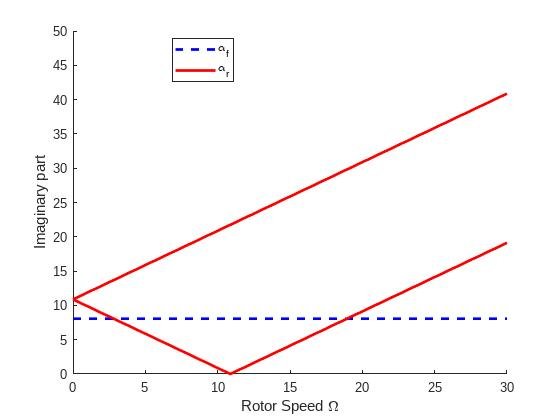
\includegraphics[width=0.7\linewidth]{gambar/Imag(uncoupled).jpg}}
	\caption{Plot grafik imajiner terhadap kecepatan rotor $\Omega$ pada kondisi \textit{uncoupled}.}
	\label{fig:imag(uncoupled)}
\end{figure}

\begin{figure}[H]
	\centering
	\fbox{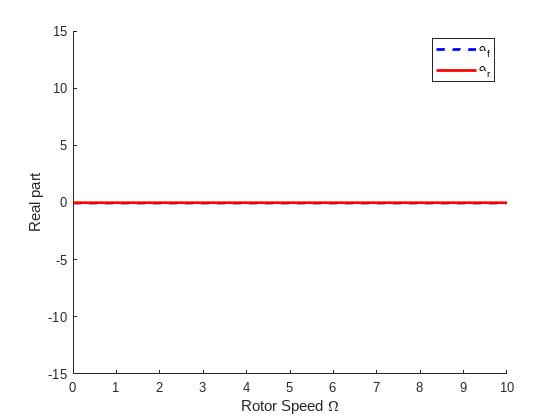
\includegraphics[width=0.7\linewidth]{gambar/Real(uncoupled).jpg}}
	\caption{Plot grafik real terhadap kecepatan rotor $\Omega$ pada kondisi \textit{uncoupled}.}
	\label{fig:real(uncoupled)}
\end{figure}

Kemudian, berikut ini adalah grafik plot untuk bagian imajiner dan riil saat sistem \textit{coupled}.

\begin{figure}[H]
	\centering
	\fbox{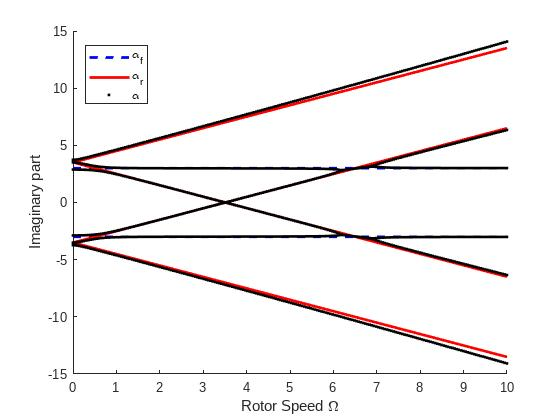
\includegraphics[width=0.7\linewidth]{gambar/Imag(coupled).jpg}}
	\caption{Plot grafik imajiner terhadap kecepatan rotor $\Omega$ pada kondisi \textit{coupled}.}
	\label{fig:imag(coupled)}
\end{figure}

\begin{figure}[h]
	\centering
	\fbox{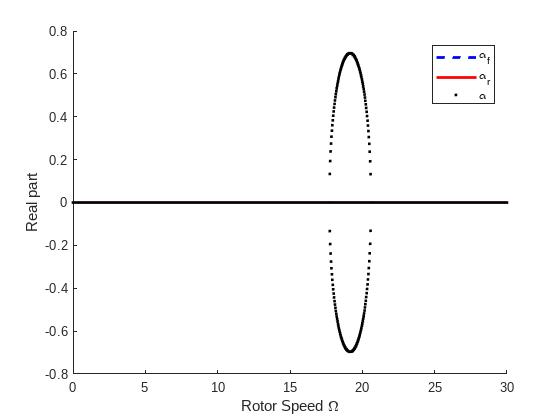
\includegraphics[width=0.7\linewidth]{gambar/Real(coupled).jpg}}
	\caption{Plot grafik real terhadap kecepatan rotor $\Omega$ pada kondisi \textit{coupled}.}
	\label{fig:real(coupled)}
\end{figure}

$\alpha_f$ merupakan nilai eigen dari \textit{fuselage} (berwarna biru dengan garis putus-putus) dan $\alpha_r$ merupakan nilai eigen dari rotor helikopter (berwarna merah). Sedangkan $\alpha$ merupakan nilai eigen dari sistem \textit{coupled}.

\section{Pembahasan}
\label{sec:pembahasan}



Identifikasi 